\documentclass[aspectratio=169]{beamer}
\usetheme{metropolis}
\usecolortheme{spruce}
\usepackage{multicol}
\usepackage{makecell,transparent}
\usepackage{graphicx}
\usepackage{soul}
\usepackage{marvosym} % Ligntning symbol

\usepackage{tikz}
\usetikzlibrary{positioning,backgrounds}

% LEAN START
\usepackage{xcolor}
\usepackage{amsmath}
\usepackage{nameref}
\usepackage{syntax}
\usepackage{hyperref}
\usepackage{fancyvrb}
\usepackage[T1]{fontenc}
\usepackage[utf8]{inputenc}
\usepackage{listings}
\usepackage{amssymb}

\usepackage{color}
\definecolor{keywordcolor}{rgb}{0.7, 0.1, 0.1}   % red
\definecolor{tacticcolor}{rgb}{0.0, 0.1, 0.6}    % blue
\definecolor{commentcolor}{rgb}{0.4, 0.4, 0.4}   % grey
\definecolor{symbolcolor}{rgb}{0.0, 0.1, 0.6}    % blue
\definecolor{sortcolor}{rgb}{0.1, 0.5, 0.1}      % green
\definecolor{attributecolor}{rgb}{0.7, 0.1, 0.1} % red

\def\lstlanguagefiles{lstlean.tex}
% set default language
\lstset{language=lean, escapeinside={<@}{@>}}

\VerbatimFootnotes

\hypersetup{
    colorlinks=true,
    linkcolor=blue,
    urlcolor=blue,
}
% LEAN END

\graphicspath{ {./images/} }

% Information for the title page
\title{A Lean Target for Lingua Franca}
\subtitle{Research Project for INF-MA-PR}
\author{\textbf{Marcus Rossel}\\[1ex] Supervisor: Christian Menard}
\institute{\textbf{Chair for Compiler Construction}\\[1ex] Technische Universität Dresden}
\date{January 1, 2023}

\metroset{block=fill}
\setbeamertemplate{footline}[page number]
\setbeamertemplate{section in toc}[sections numbered]

% Adds the table of contents before each section.
\AtBeginSection[]
{
  \begin{frame}
  \frametitle{Outline}
  \tableofcontents[currentsection]
  \end{frame}
} 

\begin{document}

% Frame: Title page
\frame{\titlepage}

%%%%%%%%%%%%%%%%%%%%%%%%%%%%%%%%%%%%%%%%%%%%%%%%%%%%%%%%%%%%%%%%%%%%%%%%%%%%%%%%%%%%%%%%

\begin{frame}{The Protagonists}
\begin{columns}[t, onlytextwidth]

% TODO: Equal height boxes?
\begin{column}{0.47\textwidth} 
\begin{block}{Lingua Franca}
  \begin{itemize}
    \item language for writing concurrent programs adhering to reactor model
    \item provides well-defined ordering and timing semantics, reducing nondeterminism
  \end{itemize}
\end{block}
\end{column}

\begin{column}{0.04\textwidth} 
\begin{center}
$+$
\end{center}
\end{column}

\begin{column}{0.47\textwidth} 
\begin{block}{Lean}
  \begin{itemize}
    \item dependently-typed functional programming language and interactive proof system
    \item allows native verification of program properties
  \end{itemize}
\end{block}
\end{column}

\end{columns}

\pause

\vspace{3mm}

\begin{center}
\textbf{But why?}
\end{center}
\end{frame}

%%%%%%%%%%%%%%%%%%%%%%%%%%%%%%%%%%%%%%%%%%%%%%%%%%%%%%%%%%%%%%%%%%%%%%%%%%%%%%%%%%%%%%%%

% TODO: Remove image background
% TODO: Add another frame with background/text coloring for the static vs. dynamic part in the code block
\begin{frame}{What is a Target?}
\begin{center}
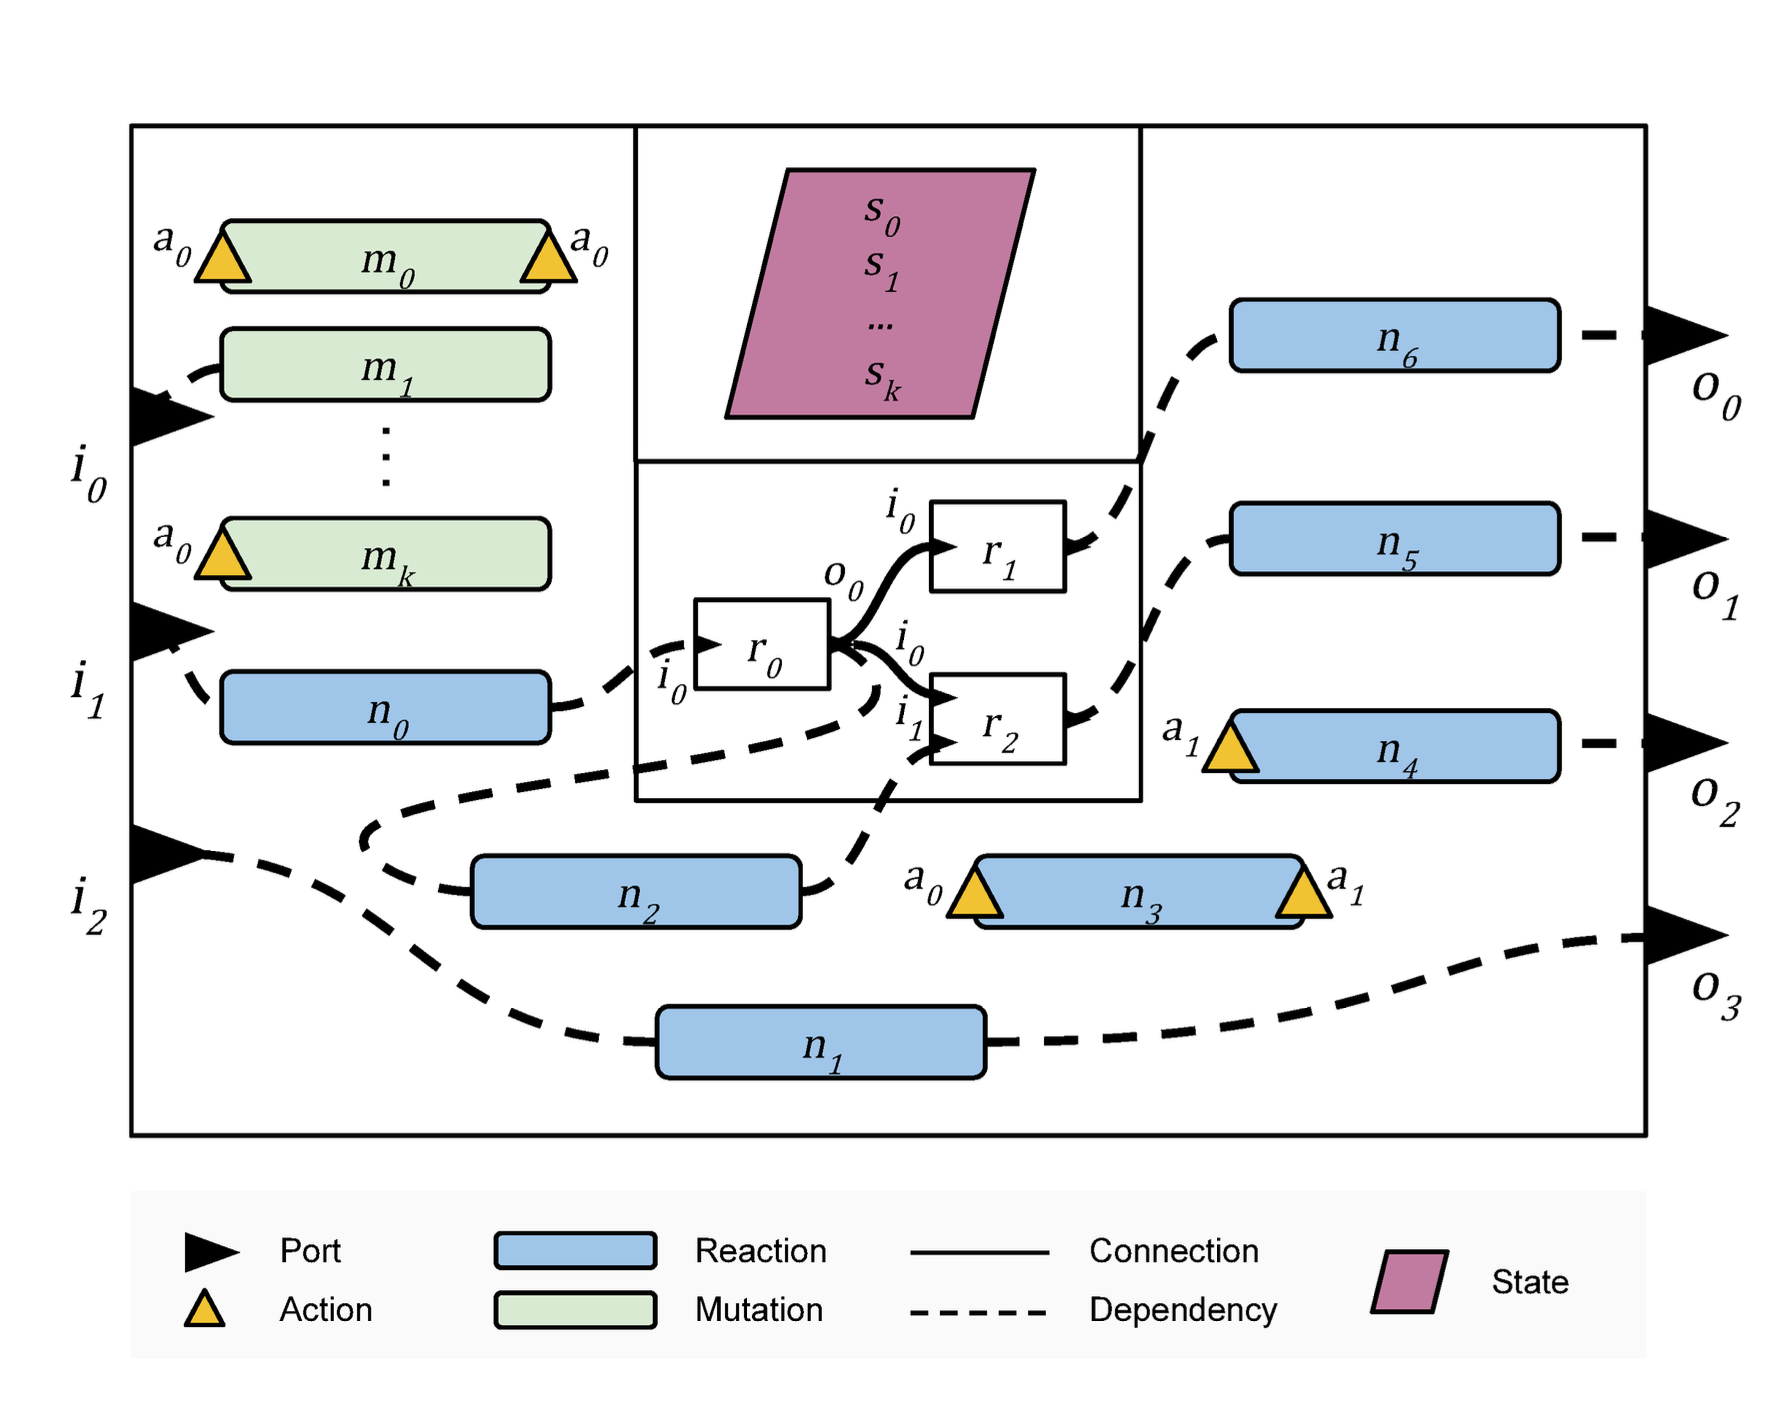
\includegraphics[scale=0.28]{reactor-overview}
\end{center}
\end{frame}

%%%%%%%%%%%%%%%%%%%%%%%%%%%%%%%%%%%%%%%%%%%%%%%%%%%%%%%%%%%%%%%%%%%%%%%%%%%%%%%%%%%%%%%%

\begin{frame}[fragile]{What is a Target?}
\begin{columns}[onlytextwidth]

\begin{column}{0.5\textwidth}
\begin{lstlisting}[basicstyle=\tiny]
reactor TestCount(start:Nat(0), stride:Nat(1), numInputs:Nat(1)) {
  state count:Nat(start)
  state inputsReceived:Nat(0)
  input x:Nat
\end{lstlisting}

\vspace{-2mm}

\begin{lstlisting}[basicstyle=\tiny]
  reaction(x) {=
    let x <- getInput .x
    let count <- getState .count
    IO.println s!"Received {x}"  
    if x != count then
      IO.println s!"ERROR: Expected {count}."
      requestStop
    setState .count <| count + (<- getParam .stride)
    setState .inputsReceived <| inputsReceived + 1
  =}

  reaction(shutdown) {=
      IO.prinln "Shutdown invoked."
      let numInputs <- getParam .numInputs 
      if (<- getState .inputsReceived) != numInputs then
        IO.println s!"ERROR: Expected to receive {numInputs}"
        requestStop
  =}
}
\end{lstlisting}
\end{column}

\begin{column}{0.05\textwidth}
\begin{center}
$\rightarrow$
\end{center}
\end{column}

\begin{column}{0.4\textwidth}
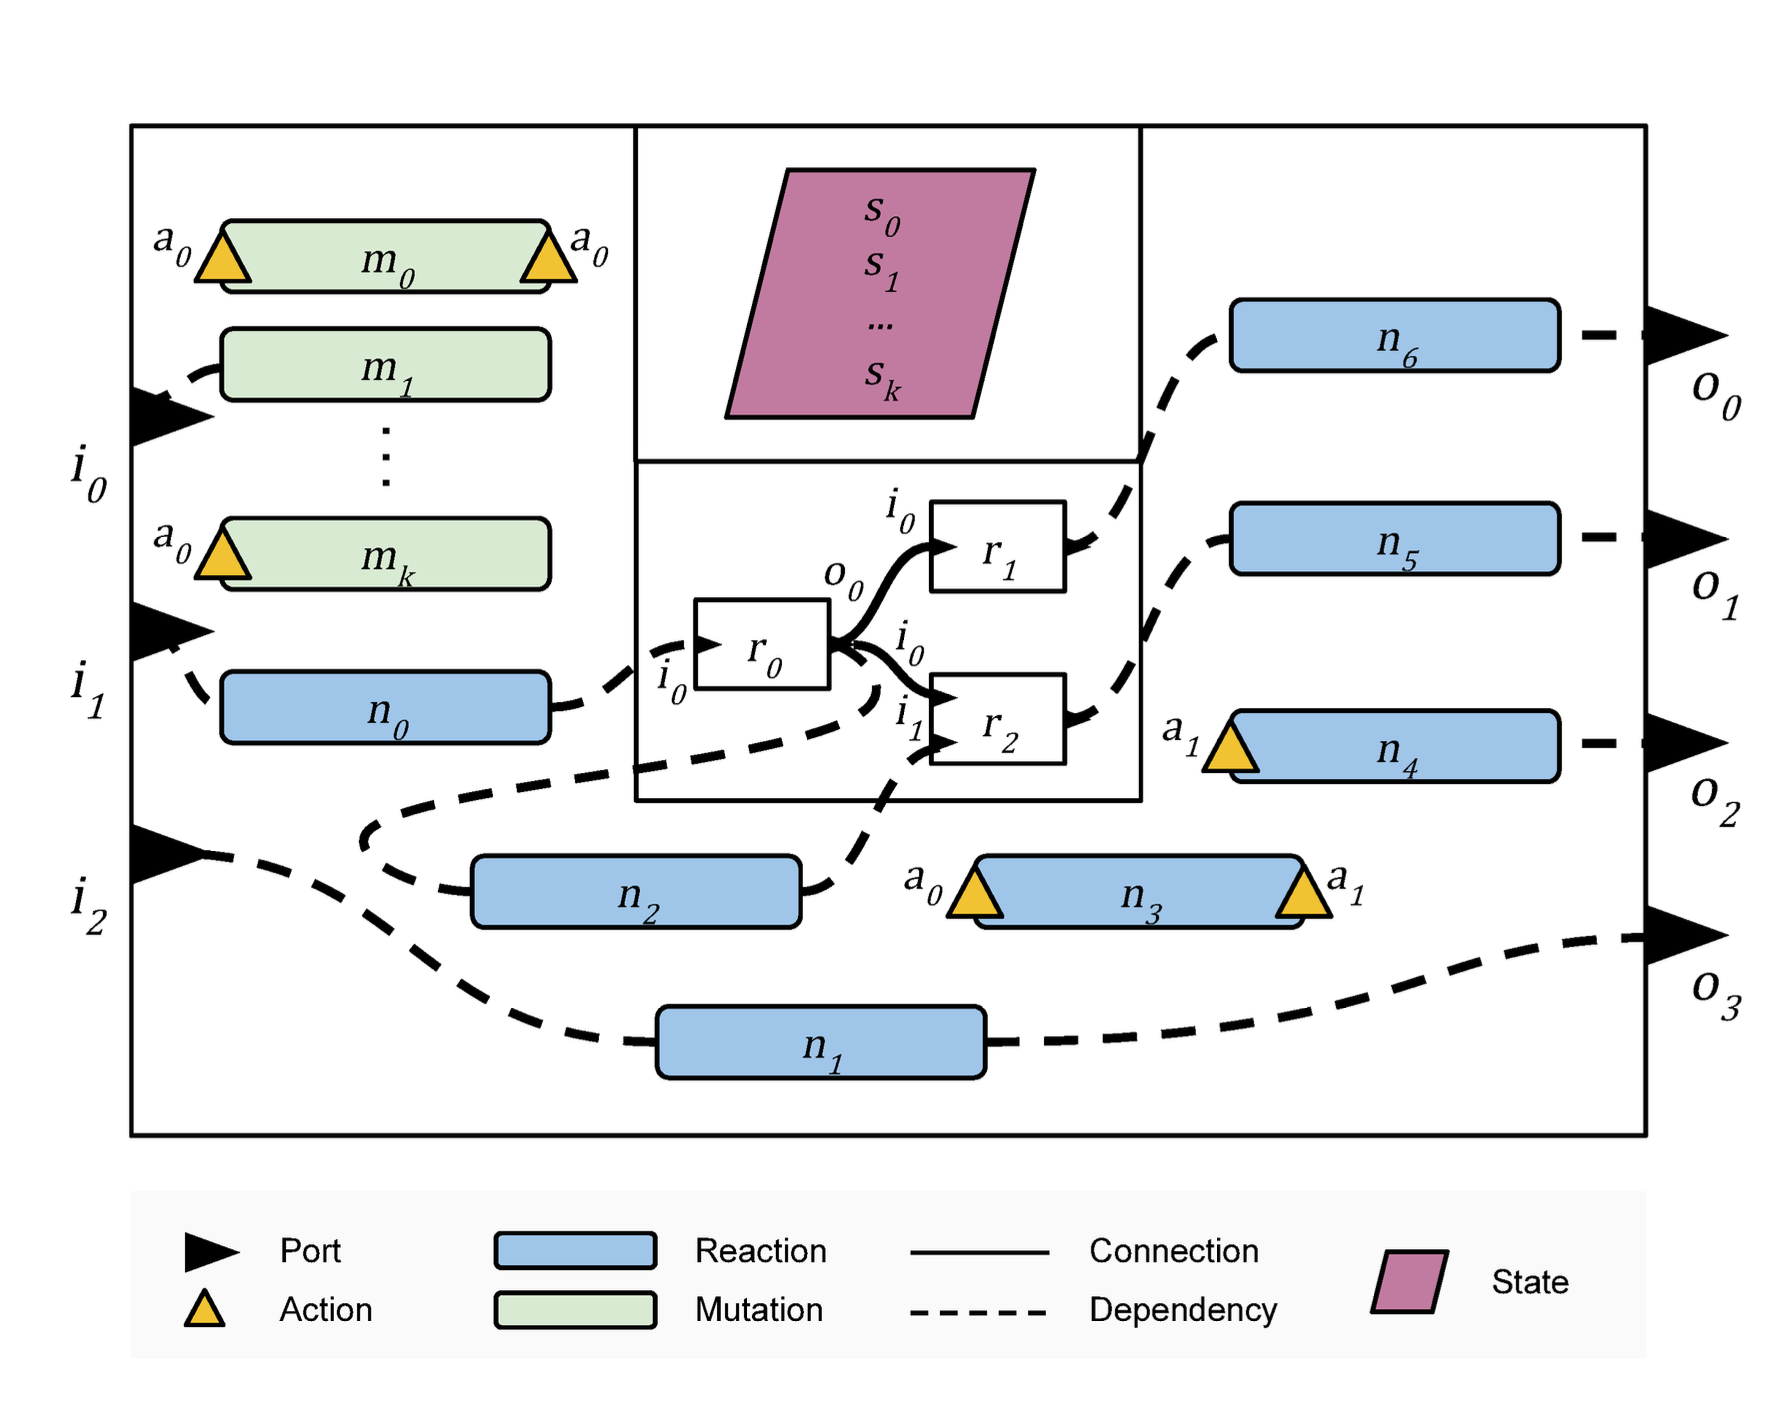
\includegraphics[scale=0.18]{reactor-overview}
\end{column}

\end{columns}
\end{frame}

%%%%%%%%%%%%%%%%%%%%%%%%%%%%%%%%%%%%%%%%%%%%%%%%%%%%%%%%%%%%%%%%%%%%%%%%%%%%%%%%%%%%%%%%

\begin{frame}[t]{What is a Target?}
... the language in which reaction bodies are written.

\pause

\vspace{5mm}

\textbf{Current Targets}

\vspace{-1.5mm}

\begin{itemize}
  \item C
  \item C++
  \item Python
  \item Rust
  \item TypeScript
  \item \textcolor{lightgray}{Lean}
\end{itemize}
\end{frame}

%%%%%%%%%%%%%%%%%%%%%%%%%%%%%%%%%%%%%%%%%%%%%%%%%%%%%%%%%%%%%%%%%%%%%%%%%%%%%%%%%%%%%%%%

\begin{frame}{Why a Lean Target?}
\begin{enumerate}
\item Add another language to the Lingua Franca target zoo.
{\transparent{0.3}
\itemsep2em 
\item How does a functional language affect runtime implementation?
\item How can dependent types be used to represent reactors?
\item What can we verify?
}
\end{enumerate}
\end{frame}

%%%%%%%%%%%%%%%%%%%%%%%%%%%%%%%%%%%%%%%%%%%%%%%%%%%%%%%%%%%%%%%%%%%%%%%%%%%%%%%%%%%%%%%%

\begin{frame}{Lingua Franca Compiler Architecture}
\begin{columns}[t, onlytextwidth]

\begin{column}{0.32\textwidth}
{\only<4->{\transparent{0.2}}
\begin{center}
\textbf{Structural Information} \\
\vspace{2mm}
$\downarrow$
\end{center}
\begin{block}{LF Frontend}
  \begin{itemize}
    \item parses LF program
    \item provides validation and functions on AST
  \end{itemize}
\end{block}
}
\end{column}

\pause

\begin{column}{0.32\textwidth}
{\only<5->{\transparent{0.2}}
\begin{center}
\textbf{Reaction Bodies} \\
\vspace{2mm}
$\downarrow$
\end{center}
\begin{block}{Code Generator}
  \begin{itemize}
    \item converts AST to target-native representation
    \item emits reaction bodies
  \end{itemize}
\end{block}
}
\end{column}

\pause

\begin{column}{0.32\textwidth}
\begin{center}
\textbf{Execution} \\
\vspace{2mm}
$\downarrow$
\end{center}
\begin{block}{Runtime}
  \begin{itemize}
    \item executes generated objects according to semantics of reactor model
  \end{itemize}
\end{block}
\end{column}

\end{columns}
\end{frame}

%%%%%%%%%%%%%%%%%%%%%%%%%%%%%%%%%%%%%%%%%%%%%%%%%%%%%%%%%%%%%%%%%%%%%%%%%%%%%%%%%%%%%%%%

\begin{frame}[fragile]{Detour: Reactor DSL}
\begin{columns}[t]

\begin{column}{0.5\textwidth}
\begin{lstlisting}[basicstyle=\small]
lf {
  reactor Server
    inputs      [inp : Int]
    outputs     [out : Int]
    actions     [err : Unit]
    state       [error : Int]
    ...
    reactions   [
      {
        kind          pure
        portSources   [inp]
        portEffects   [out]
        actionSources []
        actionEffects [err]
\end{lstlisting}
\end{column}

\begin{column}{0.5\textwidth}
\begin{lstlisting}[basicstyle=\small]
        triggers {
          ports   [inp]
          actions []
          timers  []
          meta    []
        }
        body {
          match ← getInput inp with
          | none   => schedule err 0 ()
          | some i => setOutput out i
        }
      }
    ]
}
\end{lstlisting}
\end{column}

\end{columns}
\end{frame}

%%%%%%%%%%%%%%%%%%%%%%%%%%%%%%%%%%%%%%%%%%%%%%%%%%%%%%%%%%%%%%%%%%%%%%%%%%%%%%%%%%%%%%%%

\begin{frame}{Why a Lean Target?}
\begin{enumerate}
{\transparent{0.3} \item Add another language to the Lingua Franca target zoo.}
\itemsep2em 
\item How does a functional language affect runtime implementation?
{\transparent{0.3} 
\item How can dependent types be used to represent reactors?
\item What can we do with Lean's verification capabilities?
}
\end{enumerate}
\end{frame}

%%%%%%%%%%%%%%%%%%%%%%%%%%%%%%%%%%%%%%%%%%%%%%%%%%%%%%%%%%%%%%%%%%%%%%%%%%%%%%%%%%%%%%%%

\begin{frame}{How to Execute Reactors?}

\only<2>{
``Reactors are isolated units with internal state and local functions.''

$\to$ classes with methods?

We generate an own class for each reactor and expose public methods for the reactors to update the reactor ...  
}

\only<3->{
{\transparent{0.5}
\st{
``Reactors are isolated units with internal state and local functions.''

$\to$ classes with methods?

We generate an own class for each reactor and expose public methods for the reactors to update the reactor ...  
}
}
}

\onslide<3->{
\vspace{1cm}

\textbf{Lean is functional $\to$ no classes, no mutable state, no global variables}
}

\end{frame}

%%%%%%%%%%%%%%%%%%%%%%%%%%%%%%%%%%%%%%%%%%%%%%%%%%%%%%%%%%%%%%%%%%%%%%%%%%%%%%%%%%%%%%%%

\begin{frame}[fragile]{How to Execute Reactions?}

\pause

\textbf{Goal:}

\begin{lstlisting}
  let x <- getInput .x
  let count <- getState .count
  IO.println s!"Received {x}"  
  if x != count then
    IO.println s!"ERROR: Expected {count}."
    requestStop
  setState .count <| count + (<- getParam .stride)
  setState .inputsReceived <| inputsReceived + 1
\end{lstlisting}

\end{frame}

%%%%%%%%%%%%%%%%%%%%%%%%%%%%%%%%%%%%%%%%%%%%%%%%%%%%%%%%%%%%%%%%%%%%%%%%%%%%%%%%%%%%%%%%

\begin{frame}[fragile]{How to Execute Reactions?}

\textbf{Goal: \textcolor{red}{\Lightning \, Mutable Context}}

\begin{lstlisting}
  let x <- <@\textcolor{red}{getInput}@> .x
  let count <- <@\textcolor{red}{getState}@> .count
  IO.println s!"Received {x}"  
  if x != count then
    IO.println s!"ERROR: Expected {count}."
    <@\textcolor{red}{requestStop}@>
  <@\textcolor{red}{setState}@> .count <| count + (<- <@\textcolor{red}{getParam}@> .stride)
  <@\textcolor{red}{setState}@> .inputsReceived <| inputsReceived + 1
\end{lstlisting}

\end{frame}

%%%%%%%%%%%%%%%%%%%%%%%%%%%%%%%%%%%%%%%%%%%%%%%%%%%%%%%%%%%%%%%%%%%%%%%%%%%%%%%%%%%%%%%%

\begin{frame}[fragile]{Mutable Context by Monads}

\begin{lstlisting}
def foo : Bool := ...
\end{lstlisting}

\pause

$\downarrow$ \; add ``mutable context''

\vspace{2mm}

\begin{lstlisting}
def foo' (ctx : Nat) : Nat × Bool := ...
\end{lstlisting}

\pause

$\downarrow$ \; generalize

\vspace{2mm}

\begin{lstlisting}
def ContextM (A : Type) : Type := Nat -> (Nat × A)
\end{lstlisting}

\pause

$\downarrow$ \; pretend

\vspace{2mm}

\begin{lstlisting}
def foo' : ContextM Bool := ..
\end{lstlisting}

\end{frame}

%%%%%%%%%%%%%%%%%%%%%%%%%%%%%%%%%%%%%%%%%%%%%%%%%%%%%%%%%%%%%%%%%%%%%%%%%%%%%%%%%%%%%%%%

\begin{frame}[fragile]{Mutable Context by Monads}
\begin{columns}[onlytextwidth]  

\begin{column}{0.45\textwidth}  
\begin{lstlisting}
def foo' : ContextM Bool := ...
\end{lstlisting}

\begin{lstlisting}
def bar : ContextM Bool := 
  fun ctx =>
    let ⟨ctx₁, b₁⟩ := foo' ctx
    let ⟨ctx₂, b₂⟩ := foo' ctx₁
    ...
    let ⟨ctxₙ, bₙ⟩ := foo' ctxₘ
    (ctxₙ, b₁ ∧ bₙ)
\end{lstlisting}
\end{column}

\pause

\begin{column}{0.1\textwidth}
\begin{center}
$\to$
\end{center}
\end{column}

\begin{column}{0.4\textwidth}  

\vspace{5mm}  
\begin{lstlisting}
def bar : ContextM Bool := do
  let b₁ <- foo'
  let b₂ <- foo'
  ...
  let bₙ <- foo'
  return b₁ ∧ bₙ
\end{lstlisting}
\end{column}

\end{columns}  
\end{frame}

%%%%%%%%%%%%%%%%%%%%%%%%%%%%%%%%%%%%%%%%%%%%%%%%%%%%%%%%%%%%%%%%%%%%%%%%%%%%%%%%%%%%%%%%

\begin{frame}[fragile]{How to Execute Reactions?}

\only<1>{\textbf{\textcolor{red}{\Lightning \, Mutable Context}}}
\only<2->{\textbf{\textcolor{red}{Monadic Functions}}}

\begin{lstlisting}
  let x <- <@\textcolor{red}{getInput}@> .x
  let count <- <@\textcolor{red}{getState}@> .count
  IO.println s!"Received {x}"  
  if x != count then
    IO.println s!"ERROR: Expected {count}."
    <@\textcolor{red}{requestStop}@>
  <@\textcolor{red}{setState}@> .count <| count + (<- <@\textcolor{red}{getParam}@> .stride)
  <@\textcolor{red}{setState}@> .inputsReceived <| inputsReceived + 1
\end{lstlisting}

\end{frame}

%%%%%%%%%%%%%%%%%%%%%%%%%%%%%%%%%%%%%%%%%%%%%%%%%%%%%%%%%%%%%%%%%%%%%%%%%%%%%%%%%%%%%%%%

\begin{frame}[fragile]{Reaction Monad}

\vspace{4mm}

\begin{lstlisting}
def ReactionM (α : Type) := Input → Output × α
\end{lstlisting}

\pause

\begin{columns}[onlytextwidth]

\begin{column}{0.4\textwidth}
\textbf{Bookkeeping}
\begin{itemize}
  \item input ports (read)
  \item output ports (write)
  \item state variables (read \& write)
  \item input actions (read) 
  \item scheduled actions (write) 
  \item logical tag (read)
  \item stop request (write)
\end{itemize}
\end{column}

\pause

\begin{column}{0.5\textwidth}
\begin{lstlisting}
structure Input where
  ports   : Interface?
  actions : Interface?
  state   : Interface 
  params  : Interface 
  tag     : Tag

structure Output where
  ports         : Interface?
  state         : Interface
  events        : Queue Event
  stopRequested : Bool       
\end{lstlisting}
\end{column}

\end{columns}

\end{frame}

%%%%%%%%%%%%%%%%%%%%%%%%%%%%%%%%%%%%%%%%%%%%%%%%%%%%%%%%%%%%%%%%%%%%%%%%%%%%%%%%%%%%%%%%

\begin{frame}[fragile]{Reaction Monad}
\begin{lstlisting}
<@\textcolor{red}{def reaction0 : ReactionM Unit := do}@>
  let x <- getInput .x
  let count <- getState .count
  IO.println s!"Received {x}"  
  if x != count then
    IO.println s!"ERROR: Expected {count}."
    requestStop
  setState .count <| count + (<- getParam .stride)
  setState .inputsReceived <| inputsReceived + 1
\end{lstlisting}  
\end{frame}

\end{document}

